 \documentclass[11pt]{article}


\usepackage{soul}
\usepackage{natbib}
\usepackage{hyperref}
\usepackage{bookmark}
\usepackage{graphicx}             
\graphicspath{{./Figuras/}}

\usepackage{makecell}
\usepackage[margin=1in]{geometry}
\usepackage{float}                
\usepackage{amsmath}
\usepackage{amscd}
\usepackage{amsfonts}
\usepackage{amssymb}
\usepackage{bbm}
\usepackage{booktabs}
\usepackage{nameref}
\usepackage{multirow}
\usepackage[nokeyprefix]{refstyle}
\usepackage{rotating}
\usepackage{threeparttable}
\usepackage{afterpage}
\usepackage{lscape}
\usepackage{enumerate}
\usepackage{caption}
\usepackage{subcaption}
\usepackage{epstopdf}
\usepackage{setspace}
\usepackage{svg}
\usepackage{dsfont}
\usepackage{amsthm}
\usepackage{tocloft}
\usepackage{etoc}
\usepackage{lmodern}
\usepackage{bm}

\epstopdfDeclareGraphicsRule{.tiff}{png}{.png}{convert #1 \OutputFile}
\AppendGraphicsExtensions{.tiff}

\epstopdfDeclareGraphicsRule{.tif}{png}{.png}{convert #1 \OutputFile}
\AppendGraphicsExtensions{.tif}

\usepackage{tikz}
\usetikzlibrary{shapes.geometric, arrows}
\usetikzlibrary{calc}
\usetikzlibrary{matrix}

\tikzset{ 
    table/.style={
        matrix of nodes,
        row sep=-\pgflinewidth,
        column sep=-\pgflinewidth,
        nodes={
            rectangle,
            draw=black,
            align=center
        },
        minimum height=1.5em,
        text depth=0.5ex,
        text height=2ex,
        nodes in empty cells,
%%
        every even row/.style={
            nodes={fill=gray!20}
        },
        column 1/.style={
            nodes={text width=2em,font=\bfseries}
        },
        row 1/.style={
            nodes={
                fill=black,
                text=white,
                font=\bfseries
            }
        }
    }
}


\usepackage{colortbl}

\newtheorem{theorem}{Theorem}
\newtheorem{claim}[theorem]{Claim}
\newtheorem{prop}[theorem]{Proposition} 
\newtheorem{cor}[theorem]{Corollary} 

\DeclareRobustCommand{\hlgr}[1]{{\sethlcolor{green}\hl{#1}}}


\usepackage{comment}
%para esconder columnas en tablas (enrique)
\usepackage{array}
\newcolumntype{H}{>{\setbox0=\hbox\bgroup}c<{\egroup}@{}}
\linespread{1.25}

\newcommand{\wh}{\widehat}
\usepackage{anyfontsize}

\usepackage[linesnumbered,vlined,ruled,commentsnumbered]{algorithm2e}

\DontPrintSemicolon
\newcommand{\To}{\mbox{\upshape\bfseries to}}
\usepackage{anyfontsize}
%%% HELPER CODE FOR DEALING WITH EXTERNAL REFERENCES
\usepackage{xr}
\makeatletter
\newcommand*{\addFileDependency}[1]{
  \typeout{(#1)}
  \@addtofilelist{#1}
  \IfFileExists{#1}{}{\typeout{No file #1.}}
}
\makeatother

\newcommand*{\myexternaldocument}[1]{
    \externaldocument{#1}
    \addFileDependency{#1.tex}
    \addFileDependency{#1.aux}
}

%\myexternaldocument{OA}

%%%%%%%%%%%%%%%%%%%%%%%%%%%%%%%% DOCUMENT
\begin{document}


\title{Frequent Payment \thanks{}}
\author{Joyce Sadka \and Enrique Seira \and Isaac Meza }
\date{This draft:  \today \\[2 cm]}

%\vspace{.5in}


\maketitle
\begin{abstract}
XXX 
\end{abstract}


\begin{figure}[H]
    \caption{}
    \label{det_naiveness}
    \begin{center}
    \begin{subfigure}{0.45\textwidth}
        \caption{Elapsed days}
        \centering
        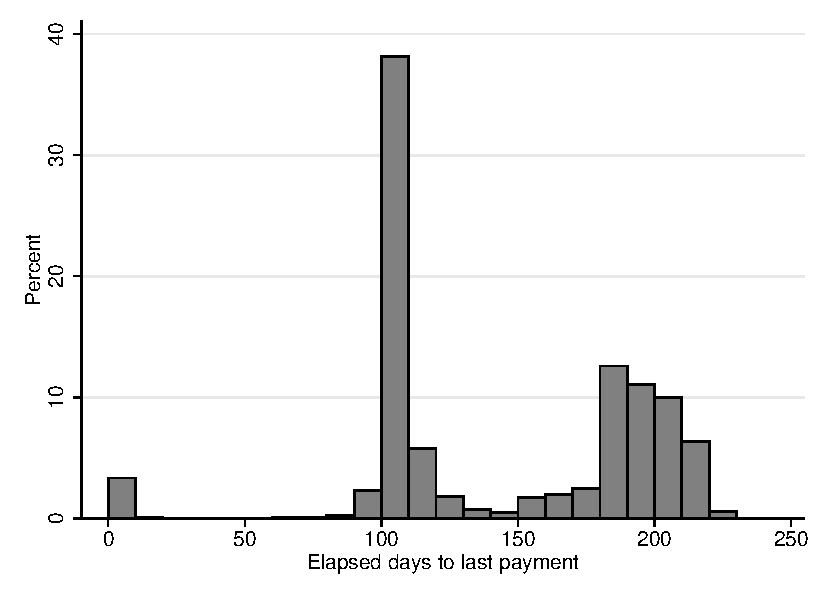
\includegraphics[width=\textwidth]{Figuras/hist_days_default.pdf}
    \end{subfigure}
        \begin{subfigure}{0.45\textwidth}
        \caption{\% of payments}
        \centering
        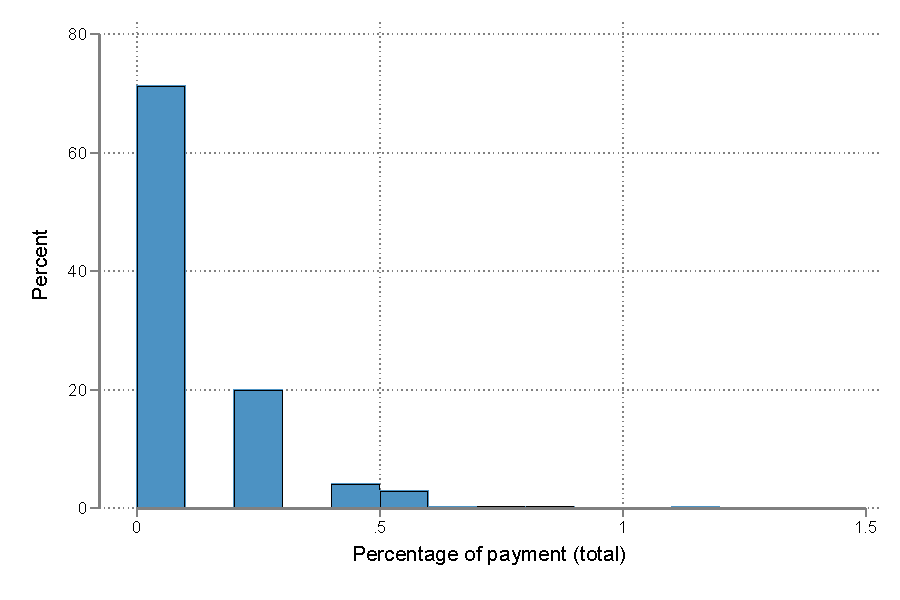
\includegraphics[width=\textwidth]{Figuras/hist_percpay_default.pdf}
    \end{subfigure}
    \begin{subfigure}{0.45\textwidth}
        \caption{Number of payments}
        \centering
        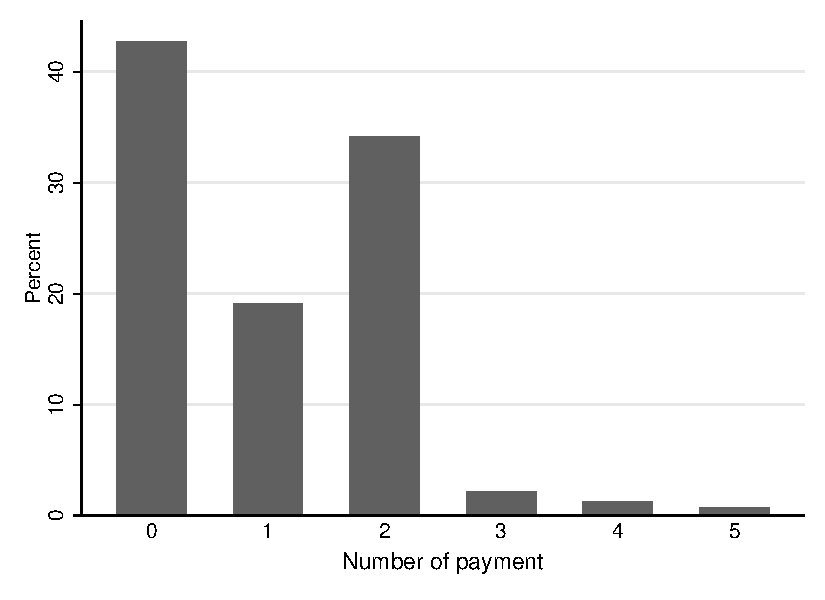
\includegraphics[width=\textwidth]{Figuras/hist_numpay_default.pdf}
    \end{subfigure}
    \end{center}
\end{figure}


\begin{figure}[H]
    \caption{Financial cost}
    \label{fc}
    \begin{center}
    \begin{subfigure}{0.45\textwidth}
        \caption{Regression}
        \centering
        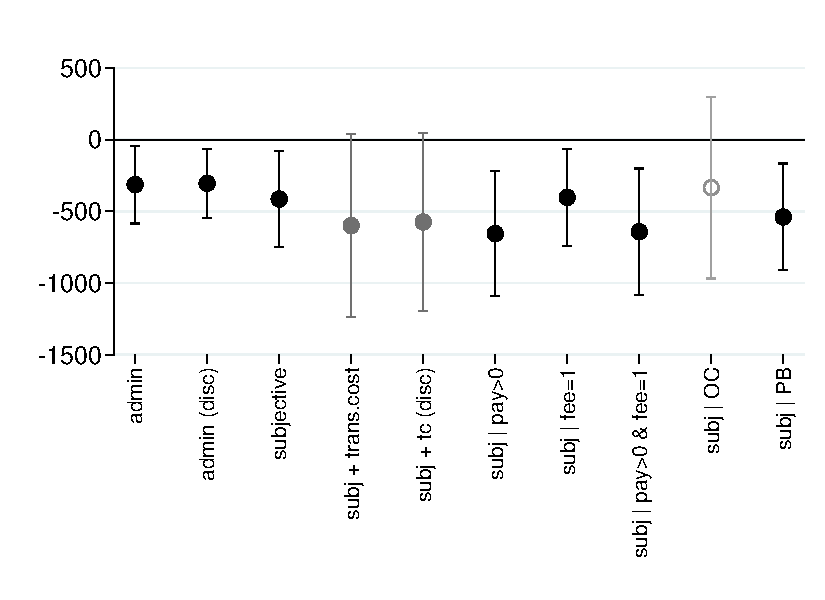
\includegraphics[width=\textwidth]{Figuras/fc_te.pdf}
    \end{subfigure}
        \begin{subfigure}{0.45\textwidth}
        \caption{Quantile regression}
        \centering
        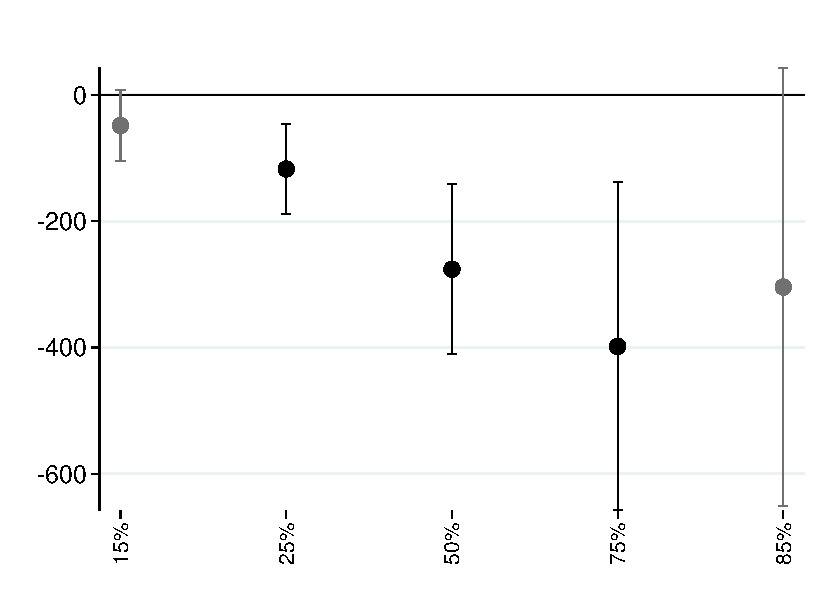
\includegraphics[width=\textwidth]{Figuras/fc_admin quantile.pdf}
    \end{subfigure}
    \end{center}
\end{figure}



\begin{figure}[H]
    \caption{Financial cost}
    \label{det_naiveness}
    \begin{center}
        \caption{Not recovery treatment effects}
        \centering
        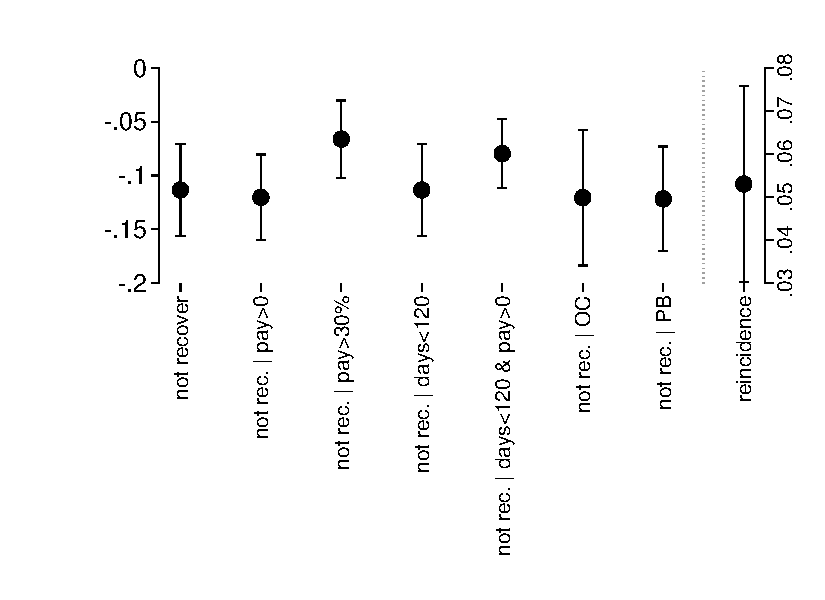
\includegraphics[width=\textwidth]{Figuras/def_te.pdf}
    \end{center}
\end{figure}


\begin{figure}[H]
    \caption{Determinants of naiveness}
    \label{det_naiveness}
    \begin{center}
    \begin{subfigure}{0.45\textwidth}
        \caption{Naiveness 1}
        \centering
        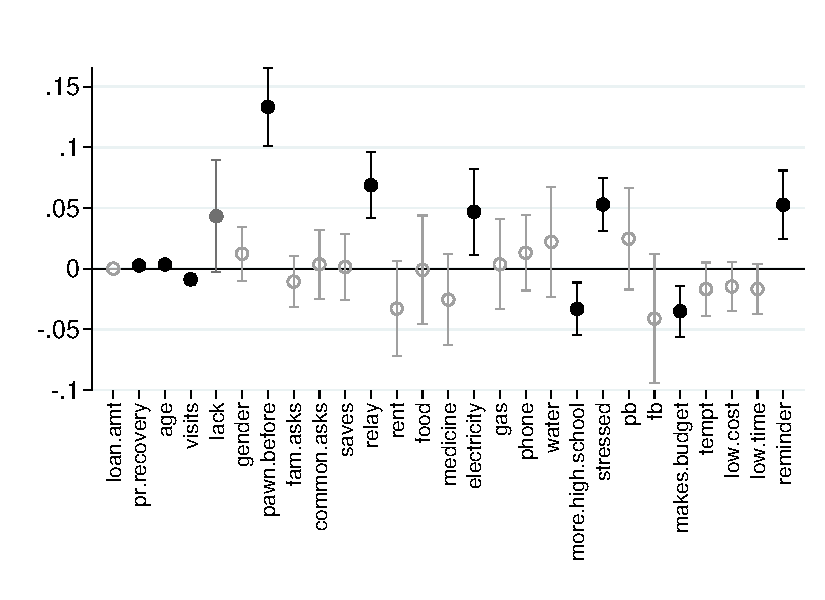
\includegraphics[width=\textwidth]{Figuras/det_naiveness_ref_c.pdf}
    \end{subfigure}
    \begin{subfigure}{0.45\textwidth}
        \caption{Naiveness 2}
        \centering
        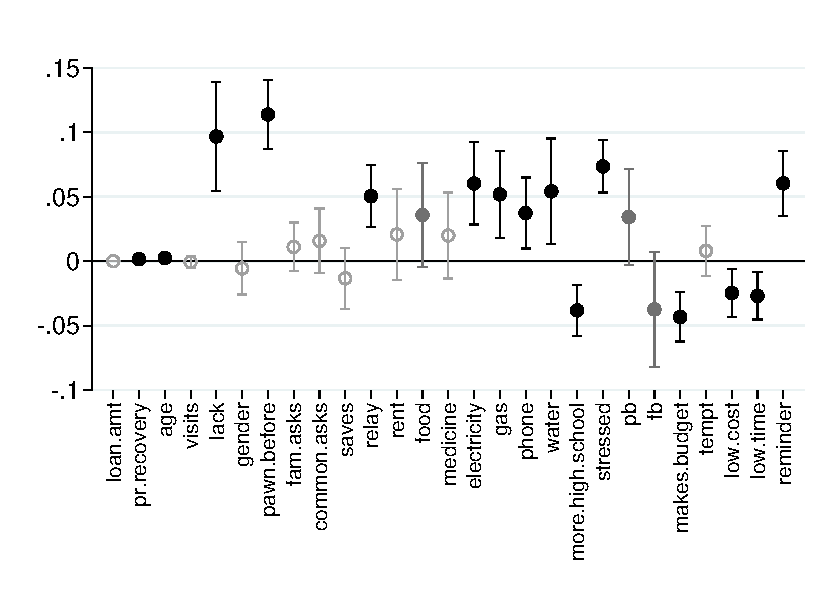
\includegraphics[width=\textwidth]{Figuras/det_naiveness_ref_default.pdf}
    \end{subfigure}
        \begin{subfigure}{0.45\textwidth}
        \caption{Naiveness 3}
        \centering
        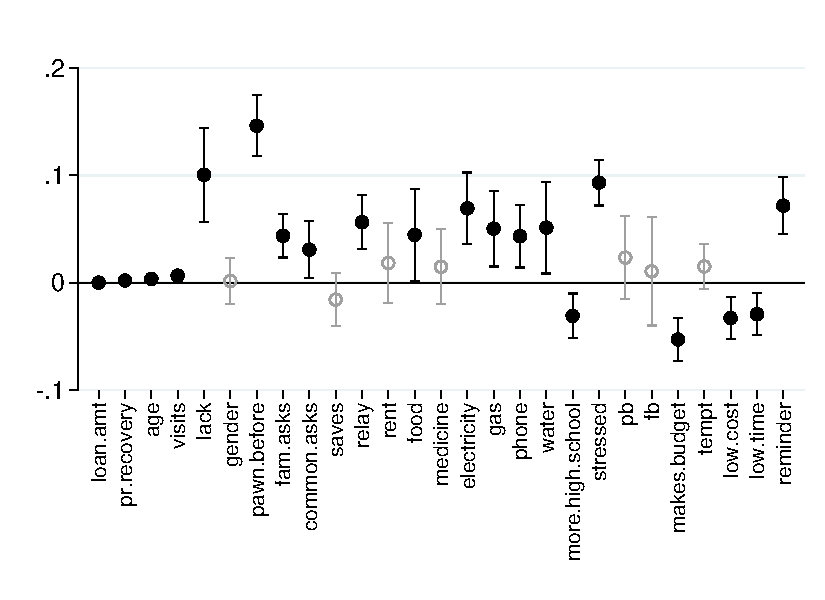
\includegraphics[width=\textwidth]{Figuras/det_naiveness_pos_pay_default.pdf}
    \end{subfigure}
    \begin{subfigure}{0.45\textwidth}
        \caption{Naiveness 4}
        \centering
        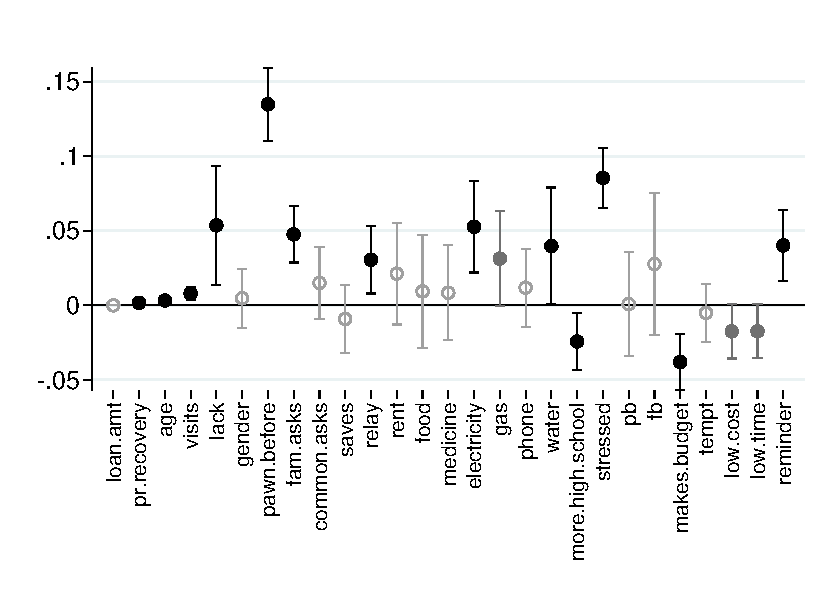
\includegraphics[width=\textwidth]{Figuras/det_naiveness_pay_30_default.pdf}
    \end{subfigure}
    \end{center}
     \footnotesize \textit{Notes: } 
      \footnotesize{ \textit{Do file: }  \texttt{naiveness.do}}
\end{figure}


\begin{figure}[H]
    \caption{Treatment effect - naiveness}
    \label{te_naiveness}
    \begin{center}
    \begin{subfigure}{0.45\textwidth}
        \caption{Naiveness 1}
        \centering
        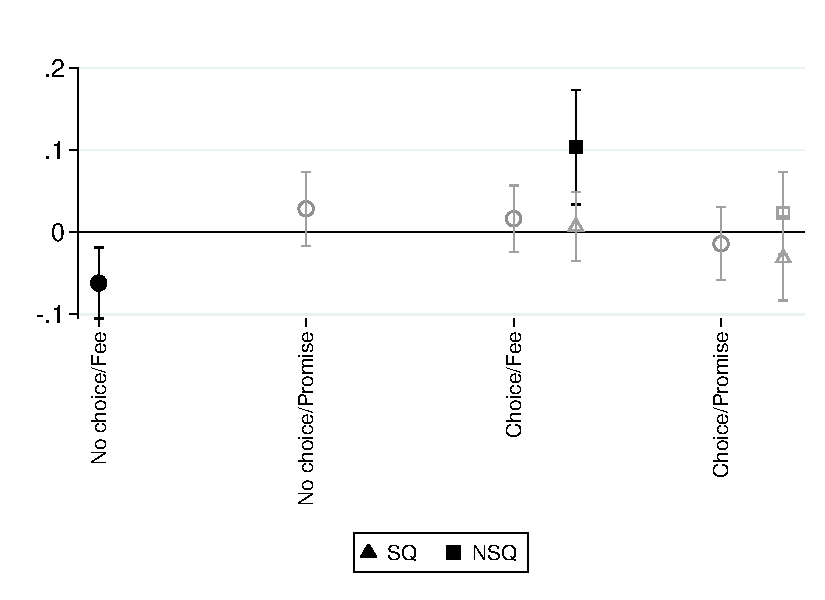
\includegraphics[width=\textwidth]{Figuras/te_graph_ref_c.pdf}
    \end{subfigure}
    \begin{subfigure}{0.45\textwidth}
        \caption{Naiveness 2}
        \centering
        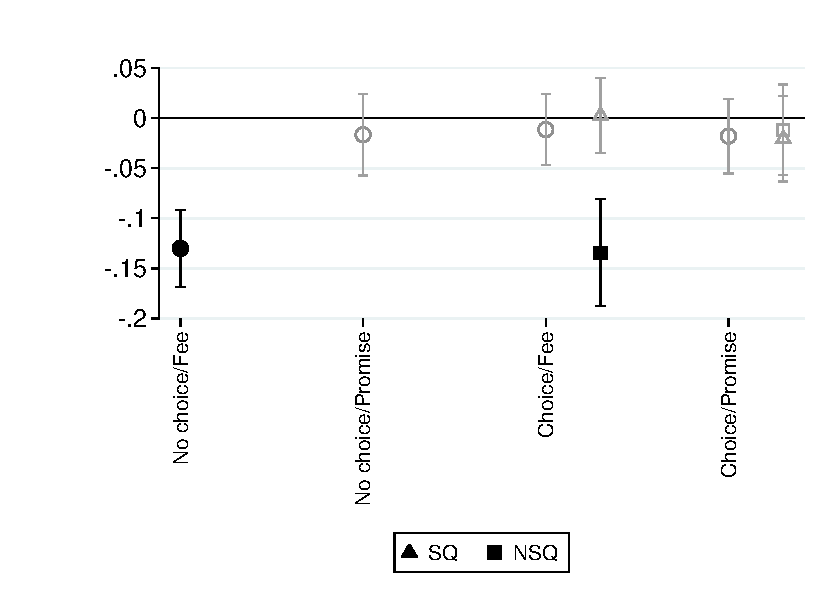
\includegraphics[width=\textwidth]{Figuras/te_graph_ref_default.pdf}
    \end{subfigure}
        \begin{subfigure}{0.45\textwidth}
        \caption{Naiveness 3}
        \centering
        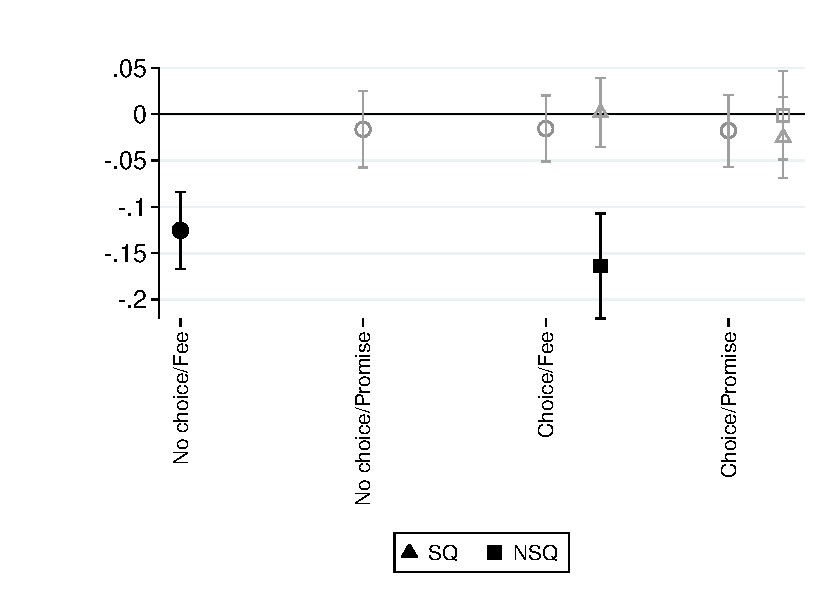
\includegraphics[width=\textwidth]{Figuras/te_graph_pos_pay_default.pdf}
    \end{subfigure}
    \begin{subfigure}{0.45\textwidth}
        \caption{Naiveness 4}
        \centering
        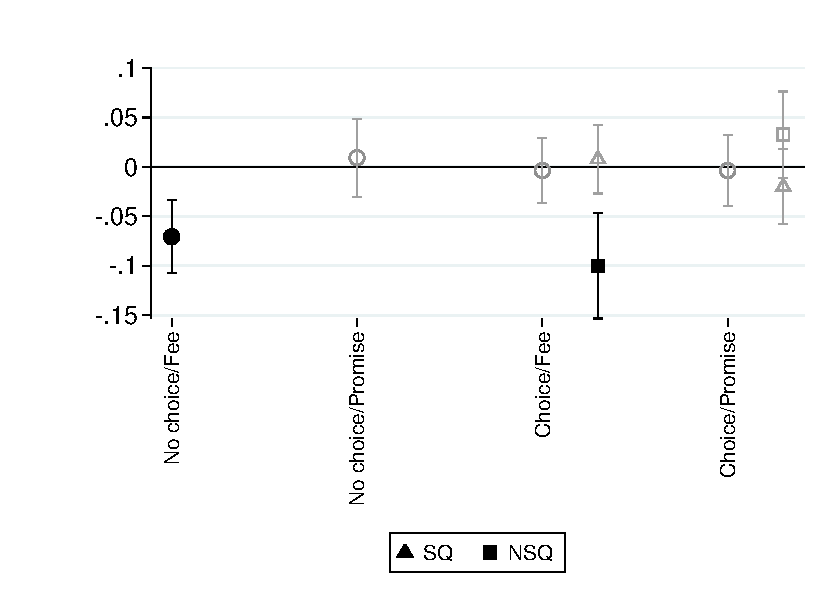
\includegraphics[width=\textwidth]{Figuras/te_graph_pay_30_default.pdf}
    \end{subfigure}
    \end{center}
     \footnotesize \textit{Notes: } 
      \footnotesize{ \textit{Do file: }  \texttt{naiveness.do}}
\end{figure}


\end{document}